\begin{wrapfigure}[22]{r}{7cm}
  \centering
  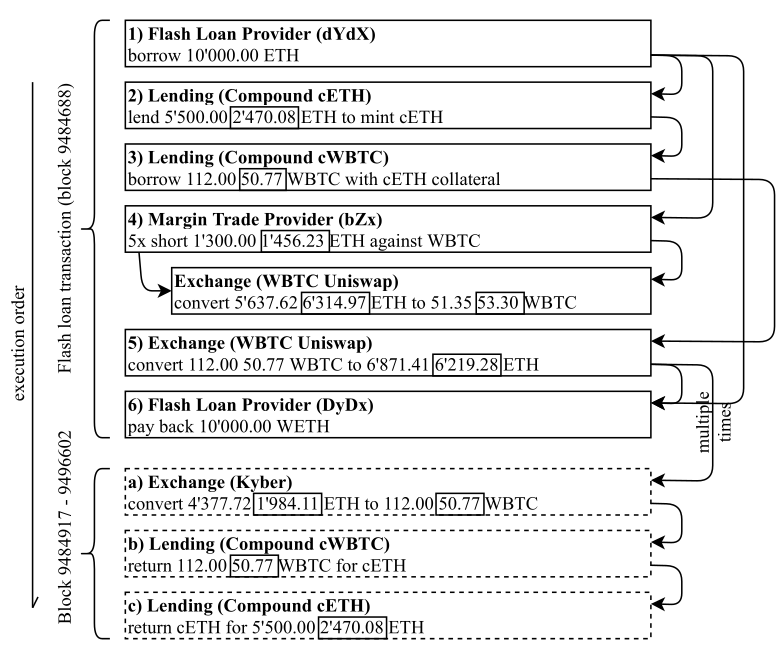
\includegraphics[width=8cm]{assests/pump-and-arb}
  \caption{This figure illustrates the pump and arbitrage
    procedure. Note that the numbers in boxes (along with the 50.77
    WBTC in step 5) should be ignored as these are not used in this
    report \cite[p. 5 fig. 6]{attack}}
  \label{fig:pumpAndArb}
\end{wrapfigure}
\paragraph{Pump and arbitrage} A visualization of this example can be
seen in figure \ref{fig:pumpAndArb}, figure \ref{fig:pumpAndArb} is
from \cite{attack} where they describe the procedure, which we will
explain here.
\begin{wrapfigure}[18]{r}{7cm}
  \centering
  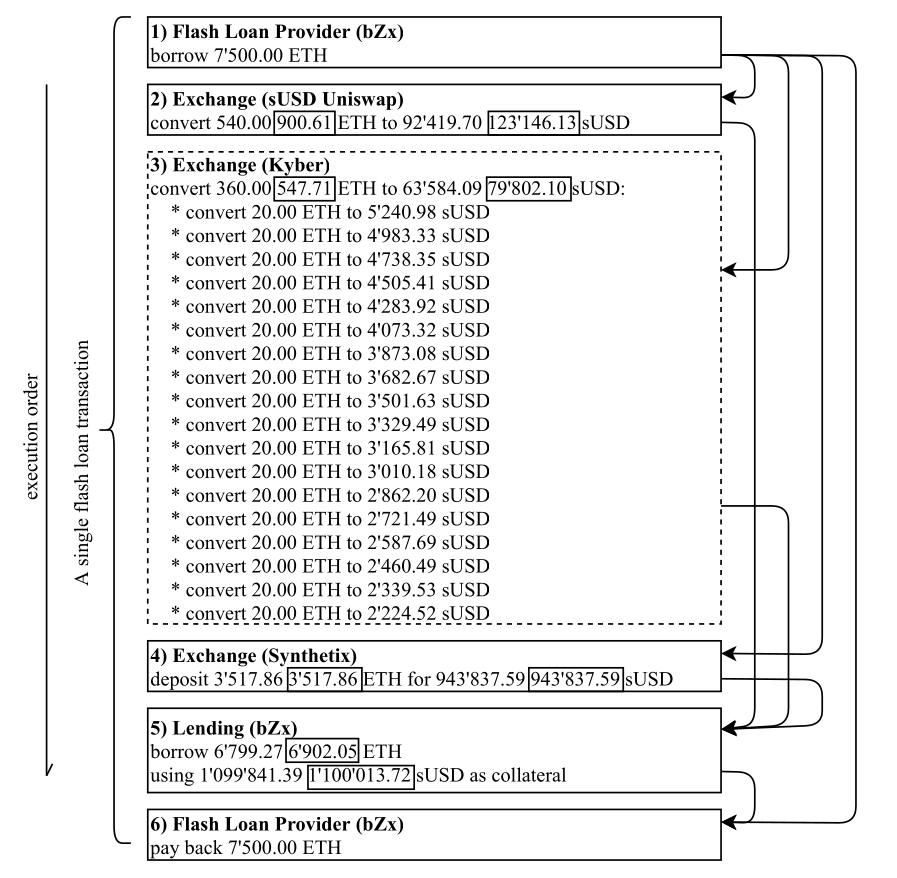
\includegraphics[width=8cm]{assests/oracle}
  \caption{This figure illustrates the oracle manipulation
    procedure. Note that the numbers in boxes should be ignored as
    these are not used in this report \cite[p. 6 fig. 7]{attack}}
  \label{fig:oracle}
\end{wrapfigure}
The main part of this trade is a margin trade on the DEX bZx to
increase the price on the Uniswap DEX. The trader uses this
manipulated price on Uniswap for arbitrage. Let look at exactly what
the trader does, by looking at figure \ref{fig:pumpAndArb}; 1) A flash
loan is taken with the trader borrowing 10,000 ETH 2) he then lends
5,500 ETH to mint 274,843.68 cETH 3) which he uses as collateral to
borrow 112.00 WBTC. 4) He then performs a margin trade, with 5x
leverage, for ETH against WBTC on bZx. When bZx receives the request
they convert 5,637.62 ETH to 51.35 WBTC, that is 109.79 ETH/WBTC on
average with a high of 124.41 ETH/WBTC, for context, at the start of
the block this transaction happened in Uniswap was at 36.55 ETH/WBTC,
this means that the price slipped from 36.55 to 124.41 that is a
slippage of $\frac{124.41-36.55}{36.55}\approx 240\%$ which both
Uniswap\footnote{This is with Uniswap v1} and bZx allows. 5) The
trader then converts the 112.00 WBTC he borrowed earlier, to 6,871.41
ETH (at 61.35 ETH/WBTC). 6) The trader then pays back the loan with
the remaining 3200 ETH from the flash loan and the 6,871.41 ETH he
just got, netting a profit off 71.41 ETH.

However this is not the real price, the real price is the
over-collateralized loan of 5,500 ETH for 112 WBTC at 49.10 ETH/WBTC
because this is fairly high so over a period of two days (steps a-c in
figure \ref{pumpAndArb}) the trader exchanges 4,377.72 ETH for 112
WBTC, at 39.08 ETH/WBTC, to redeem the 5,500 ETH thereby making 10.02
ETH per WBTC and adding in the 71.41 he made earlier the total profit
is 1,193.65 ETH. The loser here is bZx since when converting 5,637.62
ETH to 51.35 WBTC they have an average conversion rate of 109.78
ETH/WBTC, but at the time the market exchange rate was about 39.08
ETH/WBTC so they lend the trader $5,637.62-1,300=4,337.62$ ETH, but
for that they end up with 51.35 WBTC which is worth about
$51.35*39.08=2,330.86$ ETH thereby losing $4,337.62-2,330.86=2,006.76$
ETH.

\paragraph{Oracle manipulation} A visualization of this example can be
seen in figure \ref{fig:oracle}, figure \ref{fig:oracle} is from
\cite{attack} where they describe the procedure, which we will explain
here.

The main part of this trade is converting ETH to sUSD in order to
lower the price of sUSD/ETH, and then lend from a platform which uses
the conversion rate to borrow ETH at a low cost. In more detail the
trader; 1) borrows 7,500 ETH using a flash loan 2) convert 540 ETH to
92,419.7 sUDS at 171.15 sUSD/ETH (on the Kyber-Uniswap reserve), 3) he
then converts 360 ETH to 63,584.09 sUSD at 111.23 sUSD/ETH (on Kyber)
over are series of conversions. These two steps are done to
lower the sUSD/ETH price on Kyber, and 4) he converts 3,517.86 ETH to
943,837.59 sUSD and he now has a total of
$92,419.7+63,584.09+943,837.59=1,099.841.38$ sUSD 5) which he uses as
collateral to borrow 6,799.27 ETH at 162.66 sUSD/ETH on bZx, and 6)
pays back the (flash) loan to bZx.

The key point is that bZx uses Kyber as a price oracle so with the
lowered price he can now borrow a lot more ETH using the sUSD than the
normal market rates would indicate, this can be seen by the simple
calculation that he spends $540+360+3,517.86=4,417.86$ ETH to borrow
6,799.27 ETH, that is a profit of $6,799.27-4,417.86=2,381.41$ ETH. He
ends up manipulating the prices on Kyber from 268.30 sUDS/ETH to
107.83 sUSD/ETH (remember the conversion rates mentioned in the steps
are averages, while these two numbers are the highs and lows). The
loser here is bZx, they lend 6,799.27 ETH to the trader for 1,099,841
sUSD which is worth approximately 4,099.29 ETH (give an estimated rate
of 268.30 sUSD/ETH at the time), so they lose
$6,799.27-4,099.29=2,699.97$ ETH.
